\section{Vježba 2: Metoda podudaranja susjedstva piksela s modelom}

\subsection{Opis vježbe}
Učitati zadanu sliku na kojoj piše neki tekst. Mišem označiti
(kvadratićem zaokružiti) jedno slovo u tekstu na slici. Primjenom metode
podudaranja susjedstva piksela s modelom (engl. \textit{Template
Matching} potrebno je odrediti i označiti (kvadratićem zaokružiti) sva
slična (\textbf{ista}) slova poput označenog slova.

\subsection{Objašnjenje programa}

\subsubsection{Kontrola programa}

Prilikom pokretanja programa iz komandne linije potrebno je 
predati programu putanju do slike (argv[1]) u protivnom se program 
nece pokrenuti. \\

\begin{lstlisting}[language=bash,caption={Pokretanje programa iz
    komandne linije}]
$ ./template_matching ../images/tm-quick.png
\end{lstlisting}

Nakon pokretanja programa u ispisu komandne linije stoji da odaberemo
``t'' za pokretnje template matching-a. Međutim prije toga je prvo
potrebno odredit model odabirom slova ``r'' te nakon toga. Sada možemo
pritisnut ``t'' te će program izbaciti rezultate podudaranja susjedstva
piksel s modelom te označiti slične modele.
\\

\begin{lstlisting}[language=C,caption={Kontrola programa tipkovnicom}]
while (1){
    char c = waitKey(10);
    switch(c) {
        case 'r':
            cout << "Setting callback, calling cropImage  ...\n";
            setMouseCallback(imageName, onMouse, (void*)&loaded_img);
            break;
        case 't':
            if(!croped_roi.data){
                cout << "nisi cropao nista" << endl;
                break; }
            matchTemplateTrackbar( );
            break;
            } }
\end{lstlisting}

\subsubsection{Metoda podudaranje susjedstva piksela s modelom}
Kao što samo ime metode kaže uspoređuje se matrica modela \textbf{T}
(engl. \textit{template}) s matricom slike \textbf{I} na način da
model klizi preko slike. Nad svakim pikselom iz modela izvodi se
matematička funkcija. Funkcija vraća sličnost modela i uspoređenog
dijela slike. Tu vrijednost funkcija zapisuje u rezultantn matricu
\textbf{R}. Opisanu radnju izvršavamo pozivom funkcije
\textit{cv::matchTemplate()}. U toj funkciji je impelementirano šest
matematičkih metoda za pronalazak sličnosti. Svaku od njih se može
isprobati pomicanjem klizača. Nakon dobivanja rezultantne matrice
slijedi pronalazak pozicija piksela koji imaju najveću sličnost modela i
slike. To se možemo odraditi na više načina. Primjerice možemo korisitit 
funkciju \textit{cv::minMaxLoc()}. Ona nam vrati poziciju piksela s najvećom i
najmanjom vrijdnosti. Ta metoda je ograničena na vraćanje samo jednog 
sličnog rezultata. Drugi način je da nad normaliziranom rezultatnom
matricom (vrijdnosti prikazna brojevim između 0 i 1), pustimo funkciju
praga i time odbacimo slabe rezultate. Nakon toga prođemo kroz
matricu i prikažemo sve slične rezultate. Ova metoda je ograničena na
matematičke metode koje se mogu normalizirati.
\\
\begin{lstlisting}[language=C,caption={Podudaranje susjedstva piksela s
    modelom}]
void matchTemplateTrackbar( ){
    namedWindow( "source", CV_WINDOW_AUTOSIZE );
    namedWindow( "result", CV_WINDOW_AUTOSIZE );
    char* trackbar_label = "Method: \n 0: SQDIFF \n 1: SQDIFF NORMED \n 2: TM CCORR \n 3: TM CCORR NORMED \n 4: TM COEFF \n 5: TM COEFF NORMED";
    createTrackbar( trackbar_label, "source" , &match_method, max_Trackbar, matchTemplateOnCrop );
    matchTemplateOnCrop( 0, 0 );
}
void matchTemplateOnCrop( int, void* ){
    Mat source_img;
    loaded_img.copyTo( source_img );
    croped_roi.copyTo( templ_img );
    Mat gsource_img, gtempl_img;
    cv::cvtColor(source_img, gsource_img, CV_BGR2GRAY);
    cv::cvtColor(templ_img, gtempl_img, CV_BGR2GRAY);
    /// Create the result matrix
    int result_cols =  source_img.cols - templ_img.cols + 1;
    int result_rows = source_img.rows - templ_img.rows + 1;   
    result_img.create( result_rows, result_cols, CV_32FC1 );
    /// Do the Matching and Normalize
    matchTemplate( gsource_img, gtempl_img, result_img, match_method);
    normalize( result_img, result_img, 0, 1., NORM_MINMAX, -1, Mat() );
    // Remove non matching results with tresholding
    threshold( result_img, result_img, 0.8, 1., THRESH_BINARY);
    // Localizing the best match with minMaxLoc
    // Used only for testing purpose
    double minVal; double maxVal; double threshold=0.8;
    Point minLoc; Point maxLoc; Point matchLoc;
    minMaxLoc( result_img, &minVal, &maxVal, &minLoc, &maxLoc);
    rectangle( source_img, maxLoc, Point( maxLoc.x + templ_img.cols , maxLoc.y + templ_img.rows ), Scalar(0,0,255) ); 
    int x,y;
    // Go througe rows
    for (y = 1; y < result_img.rows -1; y++) {
        for (x = 1; x < result_img.cols -1; x++) {
            if (result_img.at<float>(y,x) > 0) {
                cout << y << "," << x << " = " << result_img.at<float>(y,x) << endl; 
                rectangle( source_img, Point(x,y), Point (x+templ_img.cols, y+templ_img.rows), Scalar(0,255,0));  
            } } }
    imshow( "source", source_img );
    imshow( "result", result_img);
}
\end{lstlisting}

\begin{figure}[h]
\centering
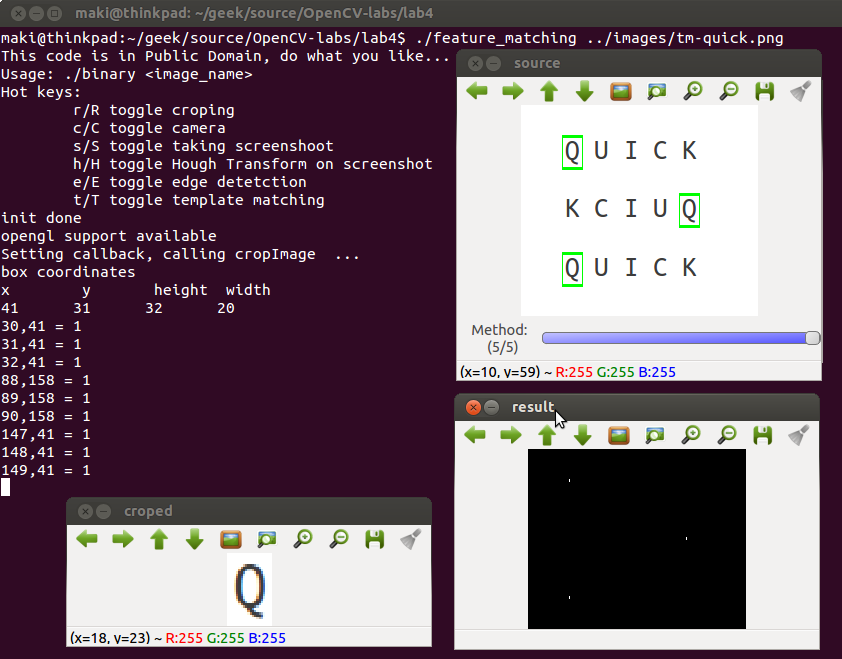
\includegraphics[scale=0.4]{images/lab2-01-tm.png}
\caption{Detekcija rubova}
\label{fig:lab2-01-tm}
\end{figure}

\subsection{Zaključak}
Glavni zadatak ove vježbe je bio pronalazk istih slova i njihova
označavanje.
Rješavanje tog problema zahtjevalo je razumjevanje rada
\textit{cv::matchTemplate()} funkcije i njenog korištenja rezultantne
matrice. Zatim je bilo bitno razumjeti kako je spremaljena rezultatna 
matrica u memoriji kako bi mogli pronaći lokacije svih sličnih modela.
Program daje dobre rezultate samo kod matematičkih funkcija koje se mogu
normalizirati, te je to područje koje se može unaprijediti.
Logika ovog programa je okosnica većine programa za optičko
prepoznavanje znakova (engl. \textit{optical character recognition}, a
postoje i mnoge druge primjene ove metode.
